\documentclass[border=10pt]{standalone}
\usepackage[svgnames]{xcolor}
\usepackage{amsmath}
\usepackage{pgfplots}
\pgfplotsset{compat=newest}
\usepackage[sfdefault]{FiraSans}
\usepackage{FiraMono}
\renewcommand*\familydefault{\sfdefault}
\begin{document}
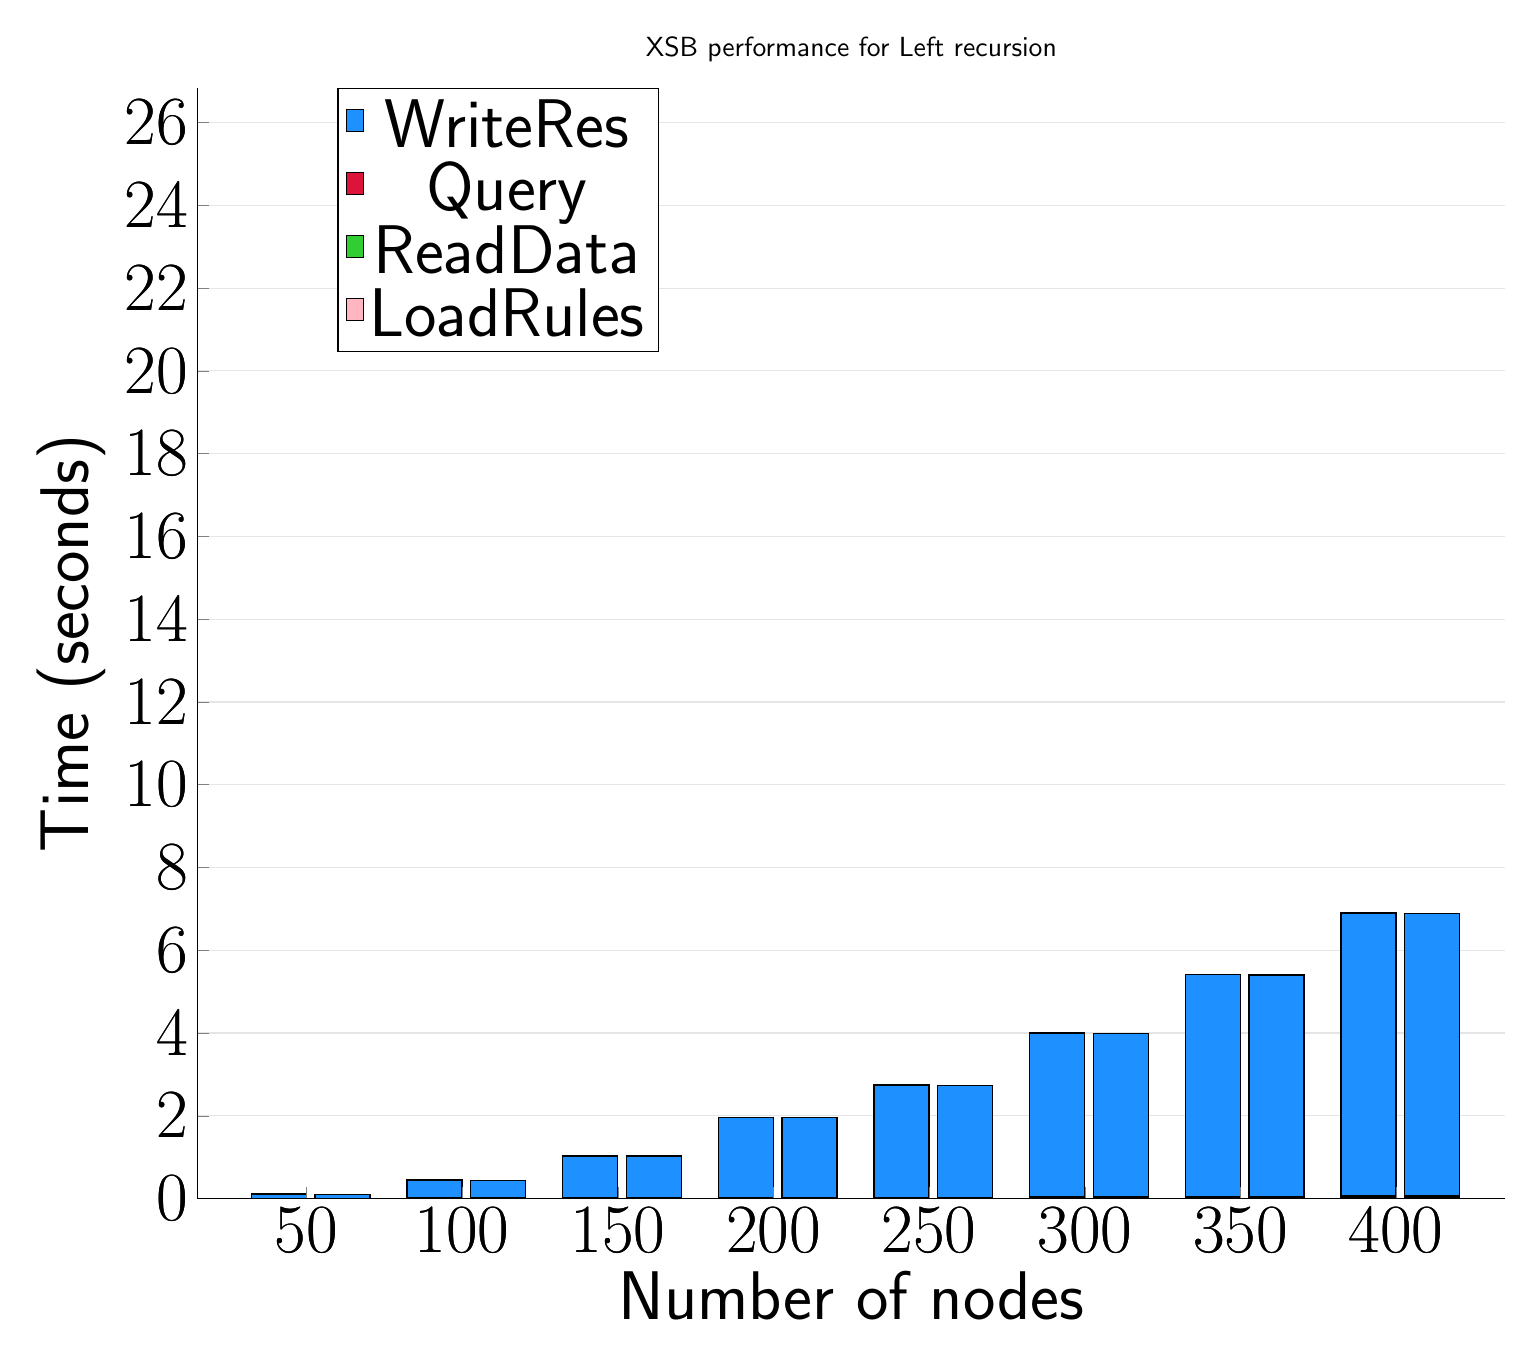
\begin{tikzpicture}
\begin{axis}[
   ybar stacked,
   title={XSB performance for Left recursion},
   bar shift=-10pt,
   width=1.5\textwidth,
   bar width=0.7cm,
   ymajorgrids, tick align=inside,
   major grid style={draw=gray!20},
   xtick=data,
   ymin=0, ymax=26.83928736050924,
   axis x line*=bottom,
   axis y line*=left,
   enlarge x limits=0.1,
   legend style={
       at={(0.23, 1)},
       anchor=north,
       legend columns=1,
       font=\Huge,
   },
   ylabel={Time (seconds)},
   xlabel={Number of nodes},
   label style={font=\Huge},
   tick label style={font=\Huge},
]
\addlegendimage{fill=DodgerBlue, draw=black, line width=0.2pt}
\addlegendentry{WriteRes}
\addlegendimage{fill=Crimson, draw=black, line width=0.2pt}
\addlegendentry{Query}
\addlegendimage{fill=LimeGreen, draw=black, line width=0.2pt}
\addlegendentry{ReadData}
\addlegendimage{fill=LightPink, draw=black, line width=0.2pt}
\addlegendentry{LoadRules}
\addplot +[fill=LightPink, draw=black, line width=0.5pt] coordinates {
    (50, 0.004652976989746093)
    (100, 0.0051076412200927734)
    (150, 0.0054800510406494175)
    (200, 0.004872719446818037)
    (250, 0.004328648249308267)
    (300, 0.004471699396769207)
    (350, 0.004713694254557294)
    (400, 0.0047646363576253235)
};
\addplot +[fill=LimeGreen, draw=black, line width=0.5pt] coordinates {
    (50, 0.0021049976348876966)
    (100, 0.0028059482574462904)
    (150, 0.004332304000854493)
    (200, 0.004560947418212893)
    (250, 0.004836400349934894)
    (300, 0.0051883061726888)
    (350, 0.006152709325154624)
    (400, 0.007227659225463864)
};
\addplot +[fill=Crimson, draw=black, line width=0.5pt] coordinates {
    (50, 0.0007483164469401043)
    (100, 0.0035746892293294272)
    (150, 0.009400606155395494)
    (200, 0.015453735987345368)
    (250, 0.0186786651611328)
    (300, 0.029425064722696934)
    (350, 0.04019792874654133)
    (400, 0.05389539400736491)
};
\addplot +[fill=DodgerBlue, draw=black, line width=0.5pt] coordinates {
    (50, 0.09967271486918157)
    (100, 0.4342617193857829)
    (150, 1.0127193133036296)
    (200, 1.9407242933909112)
    (250, 2.714004357655844)
    (300, 3.963879903157553)
    (350, 5.358935753504432)
    (400, 6.839287360509238)
};
\end{axis}
\begin{axis}[
   ybar stacked,
   bar shift=13pt,
   width=1.5\textwidth,
   bar width=0.7cm,
   ymajorgrids, tick align=inside,
   major grid style={draw=none},
   xtick=data,
   ymin=0, ymax=26.83928736050924,
   axis x line*=none,
   axis y line*=none,
   enlarge x limits=0.1,
   label style={font=\Huge},
   tick label style={font=\Huge},
]
\addplot +[fill=LightPink, draw=black, line width=0.5pt] coordinates {
    (50, 0.0032623333333333324)
    (100, 0.004868000000000001)
    (150, 0.004373666666666667)
    (200, 0.004872666666666667)
    (250, 0.0035220000000000004)
    (300, 0.004143666666666667)
    (350, 0.004025666666666667)
    (400, 0.0038170000000000005)
};
\addplot +[fill=LimeGreen, draw=black, line width=0.5pt] coordinates {
    (50, 0.0012643333333333332)
    (100, 0.0025336666666666632)
    (150, 0.0037079999999999965)
    (200, 0.004387333333333333)
    (250, 0.004609000000000003)
    (300, 0.004971333333333337)
    (350, 0.005931333333333337)
    (400, 0.006979666666666666)
};
\addplot +[fill=Crimson, draw=black, line width=0.5pt] coordinates {
    (50, 0.0005426666666666683)
    (100, 0.0034166666666666638)
    (150, 0.009353)
    (200, 0.012476333333333332)
    (250, 0.018581333333333335)
    (300, 0.029423)
    (350, 0.03970066666666667)
    (400, 0.053747333333333334)
};
\addplot +[fill=DodgerBlue, draw=black, line width=0.5pt] coordinates {
    (50, 0.09972833333333332)
    (100, 0.43118233333333333)
    (150, 1.008468)
    (200, 1.9406740000000002)
    (250, 2.7103256666666664)
    (300, 3.953121)
    (350, 5.356474666666666)
    (400, 6.824064333333332)
};
\end{axis}
\end{tikzpicture}

\end{document}
